%\documentclass[10pt,conference]{IEEEtran}
%\documentclass[9pt,conference]{sig-alternate}
%\documentclass[9pt,conference]{sig-alternate}
%\documentclass[10pt,print,letterpaper,nocopyrightspace]{sigplan-proc-varsize}
\documentclass[10pt,print,letterpaper]{sigplan-proc-varsize}

\usepackage{amsmath,epsfig}
\usepackage{url}
\usepackage{xspace}
\usepackage{colortbl}
\usepackage{subfigure}
\usepackage{dsfont}
\usepackage{boxedminipage}
\ifx\pdfoutput\undefined
\usepackage[hypertex]{hyperref}
\else
\usepackage[pdftex,hypertexnames=false]{hyperref}
\fi

\usepackage{amssymb}
\usepackage{wasysym}
\usepackage[left=2.54cm,top=2.54cm,right=2.54cm,bottom=2.54cm,nohead,nofoot]{geometry}



\DeclareMathOperator*{\argmax}{argmax}
%\usepackage{times}

\def\ucb{$^{\dagger}$}
\def\stanford{$^{\ddagger}$}
\def\arch{$^{\star}$}

\newcommand{\kb}{kB}
\newcommand{\rene}{Ren{\'e}\xspace}
\newcommand{\reneii}{Ren{\'e}2\xspace}
\newcommand{\wec}{WeC\xspace}
\newcommand{\mica}{Mica\xspace}
\newcommand{\micaii}{Mica2\xspace}
\newcommand{\micaz}{MicaZ\xspace}
\newcommand{\micadot}{Mica2Dot\xspace}
\newcommand{\iic}{I$^2$C\xspace}
\newcommand{\uA}{$\mu$A\xspace}
\newcommand{\dotmote}{Dot\xspace}
\newcommand{\mhz}{MHz\xspace}
\newcommand{\ghz}{GHz\xspace}
\newcommand{\kbps}{kbps\xspace}
\newcommand{\dsn}{DSN\xspace}
\newcommand{\io}{I/O\xspace}
\newcommand{\telos}{Telos\xspace}

\newcommand{\T}{\mathds{T}}
\newcommand{\XXXnote}[1]{{\bf\color{red} XXX: #1}}


\begin{document}

%\conferenceinfo{Sensys'08,} {November 5--7, 2008, Raleigh, NC, USA.}  
%\CopyrightYear{2008} 
%\crdata{978-1-60558-096-8/08/09} 

\title{Towards real-time, fined-grained physical data services in buildings through mobile phones}
%\numberofauthors{1} 
%\author{\alignauthor Stephen Dawson-Haggerty, Jorge Ortiz, Xiaofan Jiang and David Culler\\
%\affaddr{Computer Science Division}\\
%\affaddr{University of California, Berkeley} \\ 
%\affaddr{Berkeley, California 94720} \\
%\email{\{stevedh,jortiz,xjiang,culler\}@cs.berkeley.edu}
%} 


%\subtitle{Paper \# Insert Reg Number Here}

%\title{Alternate {\ttlit ACM} SIG Proceedings Paper in LaTeX
%Format\titlenote{(Produces the permission block, and
%copyright information). For use with
%SIG-ALTERNATE.CLS. Supported by ACM.}}
%\subtitle{[Extended Abstract]
%\titlenote{A full version of this paper is available as
%\textit{Author's Guide to Preparing ACM SIG Proceedings Using
%\LaTeX$2_\epsilon$\ and BibTeX} at
%\texttt{www.acm.org/eaddress.htm}}}
%
% You need the command \numberofauthors to handle the 'placement
% and alignment' of the authors beneath the title.
%
% For aesthetic reasons, we recommend 'three authors at a time'
% i.e. three 'name/affiliation blocks' be placed beneath the title.
%
% NOTE: You are NOT restricted in how many 'rows' of
% "name/affiliations" may appear. We just ask that you restrict
% the number of 'columns' to three.
%
% Because of the available 'opening page real-estate'
% we ask you to refrain from putting more than six authors
% (two rows with three columns) beneath the article title.
% More than six makes the first-page appear very cluttered indeed.
%
% Use the \alignauthor commands to handle the names
% and affiliations for an 'aesthetic maximum' of six authors.
% Add names, affiliations, addresses for
% the seventh etc. author(s) as the argument for the
% \additionalauthors command.
% These 'additional authors' will be output/set for you
% without further effort on your part as the last section in
% the body of your article BEFORE References or any Appendices.

\numberofauthors{2} %  in this sample file, there are a *total*
% of EIGHT authors. SIX appear on the 'first-page' (for formatting
% reasons) and the remaining two appear in the \additionalauthors section.
%
\author{
% You can go ahead and credit any number of authors here,
% e.g. one 'row of three' or two rows (consisting of one row of three
% and a second row of one, two or three).
%
% The command \alignauthor (no curly braces needed) should
% precede each author name, affiliation/snail-mail address and
% e-mail address. Additionally, tag each line of
% affiliation/address with \affaddr, and tag the
% e-mail address with \email.
%
% 1st. author
\alignauthor
%Prabal Dutta\\
%       \affaddr{Computer Science Division}\\
%       \affaddr{Univ. of California, Berkeley}\\
%       \affaddr{Berkeley, CA 94720}\\
%       \email{prabal@cs.berkeley.edu}
% 2nd. author
%\alignauthor
%David Culler\\
%       \affaddr{Computer Science Division}\\
%       \affaddr{Univ. of California, Berkeley}\\
%       \affaddr{Berkeley, CA 94720}\\
%       \email{culler@cs.berkeley.edu}
% 3rd. author
%\alignauthor
%Scott Shenker\\
%       \affaddr{Computer Science Division}\\
%       \affaddr{Univ. of California, Berkeley}\\
%       \affaddr{Berkeley, CA 94720}\\
%       \email{shenker@cs.berkeley.edu}
%}
%%%Jorge Ortiz, Yongwoo Noh, Gavin Saldanha, David Su, Jason Trager, David Culler, and Paul Wright\\
       %\affaddr{Department}\\
	%%%\affaddr{Computer Science Division}\\
       %%%\affaddr{University of California, Berkeley}\\
       %\affaddr{City, State Zip}\\
       %%%\email{jortiz@cs.berkeley.edu}
}


\maketitle

\subsection{Introduction}
The United States leads the world in per-capita energy consumption.
Our electricity use has consistently increased over the last 40 years~\cite{oecd2011} and other parts of the world are rising all 
too rapidly.  With the specter of climate change and the increasing cost of energy, we must explore new
ways for individuals to gain visibility and insight into their energy consumption in order to optimize and reduce it. 
With the increasing penetration of embedded sensors in the environment and
the continued rise in smartphone adoption, we see an opportunity for smartphones to bridge the physical world
to our computational infrastructure and provide an `energy lens' on the physical world.  

We use mobile phones to construct an entity-relationship 
graph of the physical world and combine it with streaming sensor data in order to perform detailed energy-attribution.
We limit the scope of the world to a single building domain.  We have designed and implemented a real-time, mobile energy auditing
application, called the `Energy Lens', that allows us to collect information about 
things throughout the building and how they are related to each other.  For example, computer X is inside 
room Y and connected to meter Z.  Then, we use these relationships to guide our data look-up and analytical
calculations.  For example, the load curve of room Y consists of the sum of all the power traces for loads
inside room Y.  We use the mobile smartphone as the main input tool.  Our work examines \emph{three main challenges} in setting up and 
deploying a real, whole-building infrastructure to support real-time, 
fined grained energy analytics.  

The first challenge is related to tracking and mobility.
The use of mobile phones presents classical, fundamental challenges related to mobility.  Typically, mobility
refers to the phone, as the person carrying it moves from place to place.  However, in the energy-attribution
context, we are also referring to the movement of energy-consuming objects.  Tracking their relationships to spaces 
and people is as important as tracking people.  We describe how we deal with \emph{both moving people and 
moving objects} and show that these historically difficult problems can be addressed relatively easily, if the proper infrastructure is 
in place.  %We provide evidence that the approach is simple, incrementally deployable, and scalable.

The second challenge is about capturing the inter-relationship semantics and having these inform our  analytics.
We adopt the general notion of physical tags that identify objects in the world.  Our system uses \emph{QR codes} to tag things and locations 
in the physical world.  However, \emph{any tag that provides a unqiue identifier for an object could serve the same purpose}.
Once tagged, there are three types of interactions -- 
registration, linking, and scanning -- which establish important relationships.  Registration is the act of creating a virtual object 
to represent a physical one.  Linking captures the relationship between pairs of objects.  Scanning is the act of performing an item-lookup.
Each of these interactions requires a set of swiping gestures.  Linking requires two tag swipes while the other two actions
require a single tag swipe.  Internally, we maintain a \emph{entity-relationship graph (ERG)} of things, people, and locations, that gets
updated through these sets of gestures.

The third challenge is about indoor network connectivity and access.
In order to connect these components, we rely on having `ubiquitous' network connectivity.  However, in practice, network
\emph{availability} is intermittent and our system must deal with the challenges of intermittency.  We discuss how caching
and logging are used to address these challenges.  Moreover, when connectivity is re-established, we must deal with
applying updates to the ERG, as captured by the phone while disconnected.  
% Conflicts can also occur during an update.  For example, the two updates may disagree about which items are attached
% to which meters.  We implement a very simple conflict resolution scheme, described in section~\ref{sec:conflicts}.
% Finally, certain physical-state transitions are represented as a set of updates to the ERG that must be applied 
% atomically.  We implement transactions in the log-replay and transaction manager.
% Our `Energy Lens' system is deployed in a building on our campus.  We discuss
% its architecture and our design choices.  
  
% We also discuss novel strategies for tracking moving people/things and describe how we implement these in our system.  In summary, our work
% makes the following contributions:

% \begin{itemize}
% \item We design and implement a system that captures and combines physical entities, their inter-relationships, and real-time sensor data 
% 		in buildings.% using mobile phones, qr code, and a cloud-based infrastructure.
% \item We observe that certain combinations of swipes give us useful information to set the location of people and things over time.
% 		We codify this observation in our \emph{context-tracker} and use it to maintain consistency between the entity-relationship graph and the 
% 		state of the physical world.  To the best of our knowledge, this is radically different from the approaches in standard 
% 		localization techniques.  However, we argue that it can be used to \emph{enhance} their accuracy and overall performance.
% \item We implement a prefetching algorithm to obtain context-dependent information to both improve performance and
% 		enable disconnected operation.  We also design and implement a log-replay and transaction manager over our data management layer.  We describe how different conflict-resolution policies can be implemented and our rationale for the policies we chose.
% \end{itemize}

% \vspace{0.08in}

% In the next sections we go through a motivating scenario.  We then discuss some related work, followed 
% by the system architecture, evaluation, and future directions.

\section{Related work}

%\begin{itemize}
% \item dashboard
% \item andrew's lightin control work
% \item Kamin's hvac control work
% \item BEMs
% \item sMAP stuff
%\item Buildsys 2010 work~\cite{hbci}
%\item distributed consistency management: COPS
%\item mobility: tracking things with RFID~\cite{rfid_gonz2006}
%\item mobility: tracking of people, wifi indoor localization
%\item entity-relationship graphs
%\item homeOS [microsoft]
%\item HP Cooltown~\cite{cooltown}
%\end{itemize}
Our work touches on several areas from smart home research to logistics.  In the building space, there has been
some interest in building various kinds of energy-related visual and control applications.
This work focuses on the object definition, tracking, and management component of the architecture proposed by 
Hsu et al.~\cite{hbci}.  Their work stratefied the set of challenges that one could potentially face if the application 
were deployed at scale.  Our
work, in constrast, bases its design rationale on a \emph{real deployment} that is taking place at scale in a building 
on our campus.  We focus on solving fundamental systems challenges in dealing with intermittent connectivity
and conflict resolution in tracking people and things over time.  We also focus on leveraging gestures to minimize
the cost of interaction for users, while maximizing the information we can attain about the state of the world.

% Tracking people/indoor localization
An important aspect of the Energy Lens is determining when people and things have moved.  This requires some form 
of indoor localization.  There's a large body of literature in the area of indoor localization with mobile phones ranging from 
using wifi~\cite{radar}, to sonar~\cite{cricket}, to ambient noise~\cite{abs}, and a combination of sensors on the 
phone~\cite{surroundsense, darwinphone}.  Dita~\cite{dita} uses acoustic localization of mobile phones and also uses the infrastructure 
to determine gestures in free-space that are classified into pre-defined control actions.  Each of these require relatively complex 
software and/or infrastrure.  
We take a radically different, simple approach.  We use cheap, easy to re/produce tags (QR codes), place them on things in the 
environment over incrementally and use the natural \emph{swiping gesture} that users make, when interacting with the Energy Lens 
application, to track when they have moved or when the objects around them have moved.  The working principal is to attain as much 
information from their gesture to determine when something/one has moved.  We discuss our heuristics in section~\ref{sec:swipes}.

% context-aware apps
ACE~\cite{ACE} uses various sensors on the phone to infer a user's context.  The context domain consists of a set of user activities
and semantic locations.  For example, if ACE can distinguish between {\tt Running, Driving, AtHome, or InOffice}.  ACE also infers 
the one from the others, so if the user is {\tt AtHome} then they are not {\tt InOffice}.  Energy Lens uses inference to determine
when a person or thing has moved.  Certain swipe combinations give us information about whether they moved and where they moved to or
whether an item moved and where it moved to.  The main difference is that we only infer context when a user is actively swiping, rather
than a continuous approach.  Pretching is a fundamental technique used in many domains.  However, the cost of a prefetch for mobile
application outways the benefits if the prefetched data is not useful.  Informed mobile pretching~\cite{IMP} uses cost-benefit analysis 
to determine when to prefetch content for the user.  In the Energy Lens context, we prefetch data based on their location swipes.
We also rely on pretching to anticipate loss of connectivity, not just to improve preformance.

% Tracking things
Logistic systems focus on the tracking of objects as the move through distribution sites to warehouses, stores, shelves,
and purchase.  Items are tracked through bar code or RFID readers.  However, the workload is very structured and well
defined.  The authors of~\cite{rfid_gonz2006} describe this structure and leverage it to minimize storage
requirements and optimize query-processing performance.  Energy Lens uses the QR codes as the tag and the phone as an active
reader.  As objects move, users scan those items to their new location.  However, objects may belong to one or
many people, they can be metered by multiple meters a day, and their history in the system
is on-going.  In contrast, a typical logistics workload has a start (distribution site) and end point (leaving the store
after a sale).  In our workload, relationship semantics are important; we need to know whether the meter is \emph{bound-to}
rather than simple \emph{attached-to} an item.  We discuss the difference later in the paper.
% In addition to traditional logistics-style queries -- \emph{What is the average time that it took coffee-makers to move from the 
% warehouse to the shelf and finally to the checkout counter in January of 2004?} -- energy-analytics requires queries to group
% partial traces from meter data by tracking what meters the item attached to over the specified time-frame.
% The Energy Lens system collects and manages this kind of information to enable such queries.
Furthermore, we take advatange of natural gestures the user makes with the phone while scanning QR codes to extract
information about the current location of the user or things.

% Tagging items, virtual services
The key idea in the HP Cooltown~\cite{bridgingphysical,cooltown} work is to web-enable `things' in the world, grouped-by
`place', and accessed by `people' via a standardized acquisition protocol (HTTP) and format (HTML, XML).  
Cooltown creates a web presence for things in the world either directly (embedded web server) or indirectly 
(URL-lookup tag) as a web page page that display the services it provides.  Many of the core concepts in Cooltown 
also show up in Energy Lens.  The main overlap is the use of tags in the world that contain a reference to a virtual 
resource, accessible via HTTP through
a network connection.  Cooltown, however, explicitly chooses not maintain a centralized relationship
graph, it leverages the decentralized, linking structure of the web to group associated web pages together.
Furthermore, things are assumed to not move.  People are the main mobile entities.  The kind of applications
we wish to support must track where things are and their specific inter-relationships.  We imposed a richer set of 
semantics on our, centrally maintained, relationship graph and use it to provide detailed energy information.


\section{System architecture}
The Energy Lens application aims to approximate the vision described in section~\ref{sec:vision}.  For our initial
attempt, we tagged items in a building with QR codes and allowed users to 1) register new items and tag
them with QR codes they can print from the Energy Lens site, 2) tell us which meters are attached to which items,
3) scan individual item to view their load curve over a 24-hour period.

The architecture consists of three layers: the sensing and tag layer, the data management and processing layer, and the application
layer.  In this section we discuss each layer and their most important components.  Each layer in the architecture
is carefully design to work on a real deployment with live users.  In deploying the application in a real building, we ran
into various issues that informed our design.  For example, \emph{QR code reading times vary substantially across phones
and lighting conditions}.  You must design for the least-common demoninator in terms of camera quality and lighting.

Another aspect to consider is network connectivity.  Within our building deployment, connectivity is ubiquitous, connectivity
can still be intermittent.  Connectivity may be lost for several reasons, including disassociation from an access point due
to idleness, dead spots in the building where connectivity to both wifi and 3G/4G are unavailable, multipath-induced
destructive interference, and various other reason.  Dealing with these throughout the data collection and update phase is
especially troublesome.  We discuss various mechanisms and algorithms for dealing with disconnected operation.

\subsection{Sensing and tag layer}
We deployed 20 ACme power meters~\cite{acme} on a single floor of a building on campus.  The data was made available through
sMAP~\cite{smap} and forwarded through our processing and data management layer, StreamFS~\cite{streamfs}.  We distributed
the ACmes throughout a single floor in our building and registered various plug loads as being measured by them.  We also tagged
hundreds of items and locations throughout the entire building.  In addition to tagging the 20 ACmes and the plug-loads they are
attached to, we also tagged 351 unmetered items and 139 rooms with QR codes.

\subsubsection{QR code design}
\label{sec:qrc}
QR codes must be designed to minimize scanning time.  As we iterated through various designs we noticed that dim lighting conditions
and poor cameras on certain phones caused the scan time to increase significantly.  The variance in scan time was high and
very frustrating to deal with.  Without correcting this, occupants will not engage with the application, behavior similar to attaining
user engagement on the web.

% \subsubsection{Usability (Strong dependence of occupants/users)}
% \begin{enumerate}
% \item Minimal number of swipes (protocol description)
% \item minimal amount of textual input (protocol description)
% \item piggy-backed movement classification of people and objects. (protocol description)
% \item QR code engineering to minimize swipe time (swipe times)*
% \end{enumerate}



% A QR code is a two-dimensional barcode that may encode almost 3000 bytes of data.  QR code generators
% can be found on the internet~\cite{qrcgen1, qrcgen2}.  
% Extending the approach in \cite{hbci}, in
% our
% architecture the QR code contains a meaningful {\tt URL} that a
% generic browser can access to provid ea human readable document with complete
% information about the item or space, as well as the additional
% information to bootstrap the smartphone to optimized access, such as
% native apps for interacting with the item or space.  Secondly, the 
% {\tt URL}  must be easily transformed into one that will yield a
% programmatic document, such as a JSON object, that apps can
% manipulate.  And finally, the representation of the URL itself can be
% parsed and utilized locally by native apps, typically by lookup, to
% permit rapid interaction with the item or space.

% \begin{figure}[htb!]
% \begin{center}
% 
\includegraphics[scale=0.3]{figs/qrcex}
% \caption{This is an example QR code from our deployment. This label resolves to {\tt http://tinyurl.com/6235eyw}.
% QR codes like these are used as tags physical objects and spaces/locations.}
% \label{fig:qrcex}
% \end{center}
% \end{figure}

Figure~\ref{fig:qrcexcomp} shows an example QR code used in our deployment.  Tags like these are placed on physical
objects and spaces throughout the building to link between the physical world and our virtual representation of it.
QR codes are cheap to produce.  Any printer and some tape can be used to tag an item.  This is important for scalability.
With the number of physical objects and places (floors, rooms) in a typical building, {\bf we must rely on the occupants
to scale our deployment}. Because QR codes are easy to produce, we can provide occupants with a webpage that
that produces them.  They print them out, place them on items or
places they want to interact with, register them, and provide useful
information about them.

Generating the right kind of QR code is important.  It is trivial to
encode information onto them, but it is
not trivial to design them so that they encode just enough information to be useful.  If 
too much information is encode the camera takes a long time to scan them, especially under poor lighting
conditions.  This can easily frustrate and drive away users, who are critical for scalability.
We also want to design them for the lowest common denominator in terms of camera quality.  Older
phones with cheap cameras should also be able to scan the tags quickly.  We ran some experiments to show
how complex QR codes differ from the one we design and discuss these results in Section~\ref{sec:qrcexcomp}.

\subsubsection{QR code swipe times}
\begin{figure*}[htb!]
\begin{center}
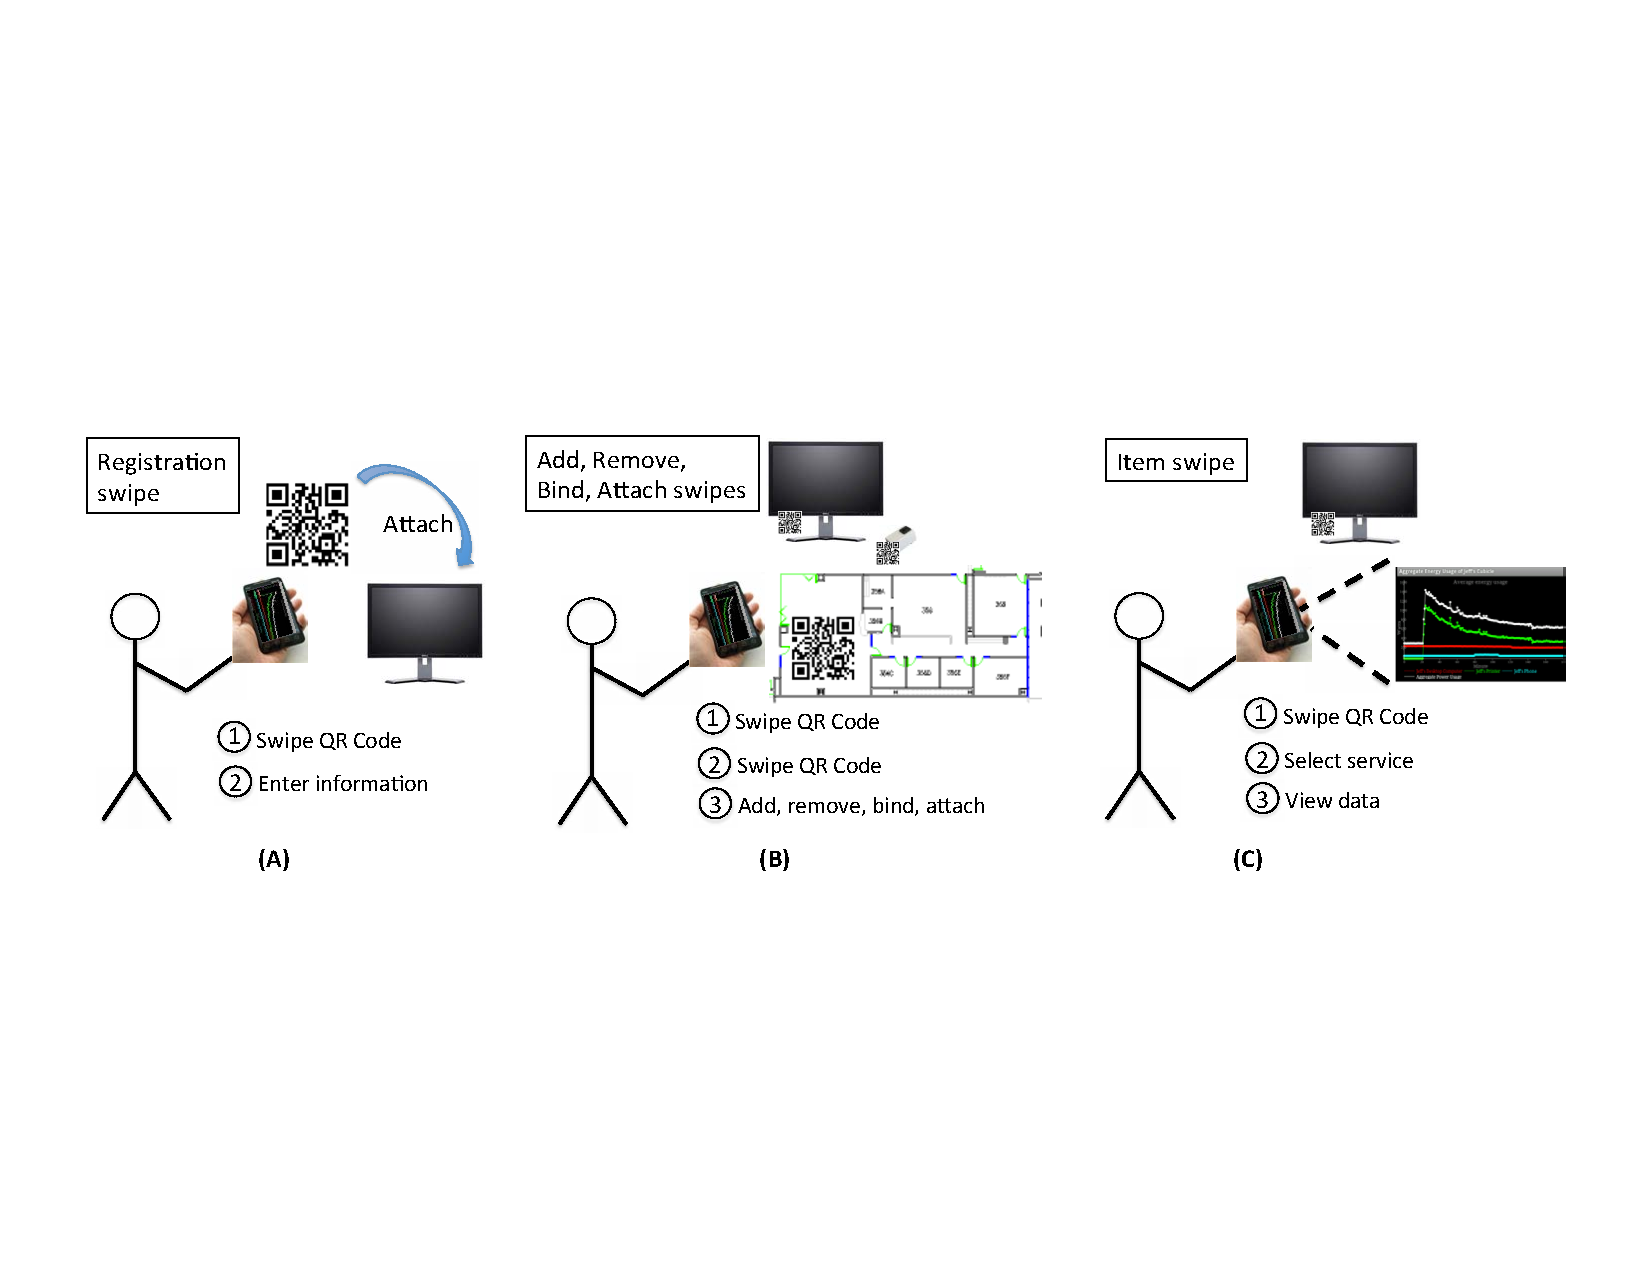
\includegraphics[width=\textwidth]{figs/swipes}
\caption{Gestures. Lorem Ipsum is simply dummy text of the printing and typesetting industry. Lorem Ipsum has 
been the industry's standard dummy text ever since the 1500s, when an unknown printer took a galley of 
type and scrambled it to make a type specimen book.  }
\label{fig:gestures}
\end{center}
\end{figure*}

\begin{figure}[htb!]
\begin{center}
\subfigure[Long QR Code.]{%
            \label{fig:qrcexfirst}
            
\includegraphics[scale=0.148]{figs/qrcexlong}
        }
\subfigure[Minimized QR Code.]{%
            \label{fig:qrcexsecond}
            
\includegraphics[scale=0.35]{figs/qrcex}
        }
\end{center}
\caption{
	The QR code on the left resolves to the same {\tt URL} at the right one, after resolution and
	redirection is complete. 
	The short label resolves to {\tt http://tinyurl.com/6235eyw}.  The second encodes about half
	the characters as the first.
	We used tinyUrl to reduce the QR code image complexity and scan time.
     }%
\label{fig:qrcexcomp}
\end{figure}

\begin{table}
\label{tab:qrscans}
\begin{center}
  \begin{tabular}{| r | c  c | }
    \hline
    			 & {\bf Average (sec) } & {\bf Variance (sec)} \\ \hline
    Short,light & 1.66 & 0.33 \\ \hline
    Short, dark & 2.08 & 0.35 \\ \hline
    Long, light & 2.26 & 0.71 \\ \hline
    Long, dark & 2.82 & 0.50 \\
    \hline
  \end{tabular}
\caption{Shows the time to scan a long QR code versus a short QR code in light and dark conditions (loosely defined).
Notice that short QR codes scan faster and with less variance that long ones.}
\end{center}

\end{table}

Table~\ref{tab:qrscans} shows the results of some simple scanning experiment between the two tags
shown above.  We scanned each QR code under light and dark lighting conditions, off the screen of my laptop.
Each experiment was run 10 times and the table shows the statistical
overview of the results. 
Clearly, scanning the simple QR code under well-lit conditions
performed the best.  The complex QR code under the same condition takes about 28-36\% longer to scan.
On a generic QR code scanner, as used here, there is a portion of the
scan time that is independent of the code complexity.  As these are
more heavily used, this is expected to be reduced substantially and
the difference is acquisition complexity will be even more pronounced.
Perhaps even more important is the variance.  Notice that the variance with the simple QR code is much smaller and
more stable under either condition.  In our experience, {\bf large variance in scan time is a major
problem for complex QR codes}.  Thus we decided to re-design our codes and push more information in the lookup
processes, as network access was more reliable than the focus of the camera on various mobile devices.
Tags are placed on all types of devices in all kinds of locations with varying degrees of lighting.
Simple QR codes are vital for widespread use.

The design choice forced us to examine others that were related.  Not being able to encode much information on 
our QR codes means we are more reliant on the network to provide the bulk of the information, to be very reliable,
and to be widespread enough that disconnection is not problematic.  Moreover, there are a number of clients
that can be used to access and display the information and the tag has to be meaningful for both.
In order to meet these criteria we (1) shrunk {\tt URL}'s using tinyURL~\cite{tinyurl} as a level of 
indirection and 
(2) designed two classes of applications: \emph{shallow} applications, and \emph{deep-inspection} applications.  Shallow
applications interact with the web-application directly while deep-inspection application use
the {\tt URL} of the web application to extract a unique identifier and provide deeper inspection
and update capabilities of the entity-relationship graph.

An example {\tt URL} we used in our deployment is {\tt http://tinyurl.com/6235eyw}.
When this is resolved, we get an empty response in the body, but we use the header to identify the QR code identifier 
that we associate with the item.  The response header looks as follows:
\begin{figure}[htb!]
\begin{center}
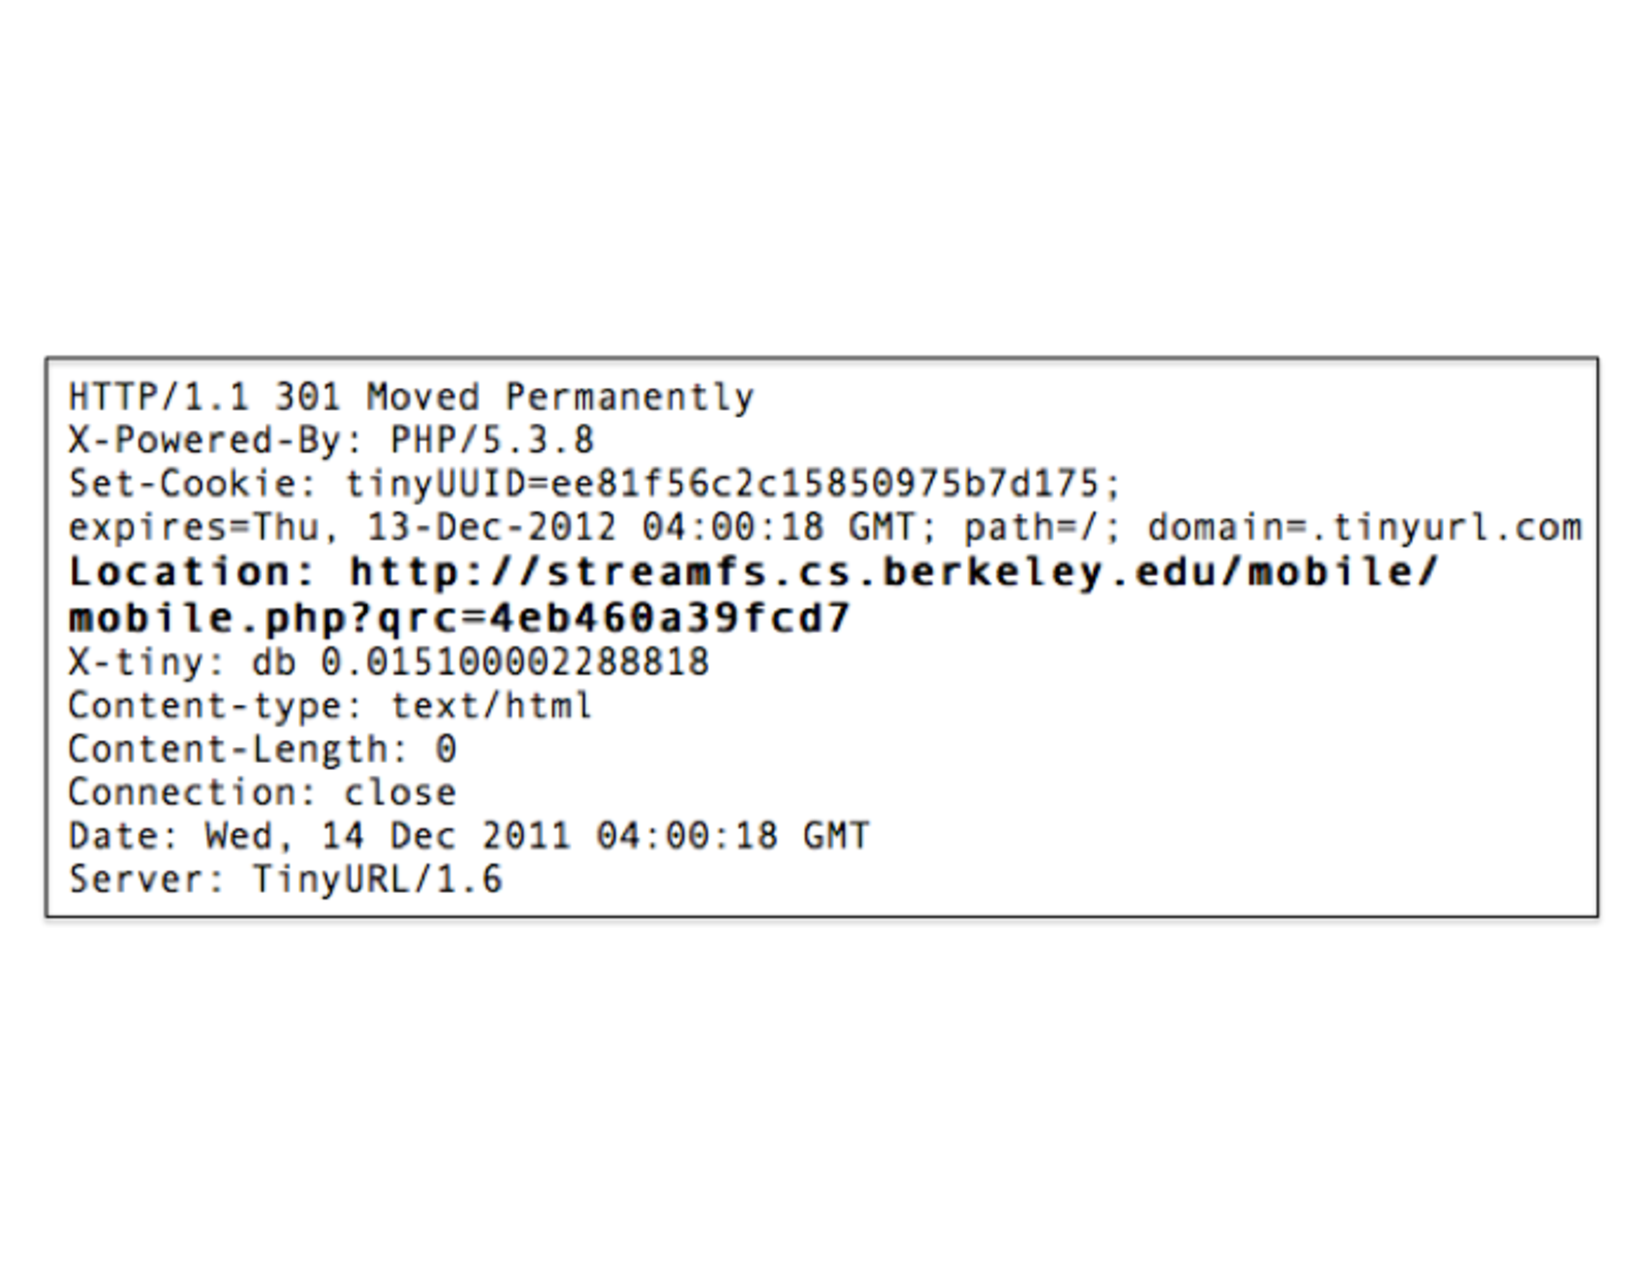
\includegraphics[scale=0.30]{figs/tinyurlhdr}
\caption{The header of the response from the {\tt tinyUrl} when resolving a QR code.  The `Location' attribute
is used to extract the unique identifier for the object this QR code tags.  It is also used to re-direct
users without the phone application to a meaningful web address for the object.}
\label{fig:tinyurlhdr}
\end{center}
\end{figure}

% It provides a web address for users to re-direct to and find information and various read-only services for the object.  However, because
% the {\tt URL} also contains a unqiue identifer \emph{qrc}, it can be used to provide for sophisticated services and capabilities.
% An example is the ability to change the virtual structure of inter-relationship between this object and other objects.  This
% is demonstrated in our energy auditing application discussed in detail in section~\ref{sec:eaudit}.
% Once items are tagged, they can be added and removed by swiping the tag and pressing the button for what you want to do with
% the item.  You also check into locations either explicit with a location-tag swipe or implicitly with an item swipe.

Notice the `Location' attribute in the header.  This is the location of the re-direct.  \emph{Shallow} applications
use the {\tt URL} directly.  The \emph{qrc} {\tt URL} is unqiue identifier for the item that this tag is attached to.
A shallow application can obtain mostly read-only service through our web applications.  For example, we'll see how
to get either item-specific data or item-aggregated data with respect to the user making the request (i.e. the total
energy consumed by \emph{my} devices).  \emph{Deep-inspection} applications are native to the phone, so we can do much
more with the tag.  Our energy auditing application allows you to related the item to other items by maintaining state of swipe
history.  This is more difficult with the web-applicaiton.  We can also use the tag and item information to couple it with
sensor information coming from sensors on the phone itself.  For example, we could determine the direction an object
is pointing by using the phone's directional sensor and negating their direction (i.e. phone is facing east, tag on item must
be facing west).






\subsection{Data management layer}

\subsection{Application layer}


\subsection{Disconnected operation}


\begin{figure}[htb!]
\begin{center}
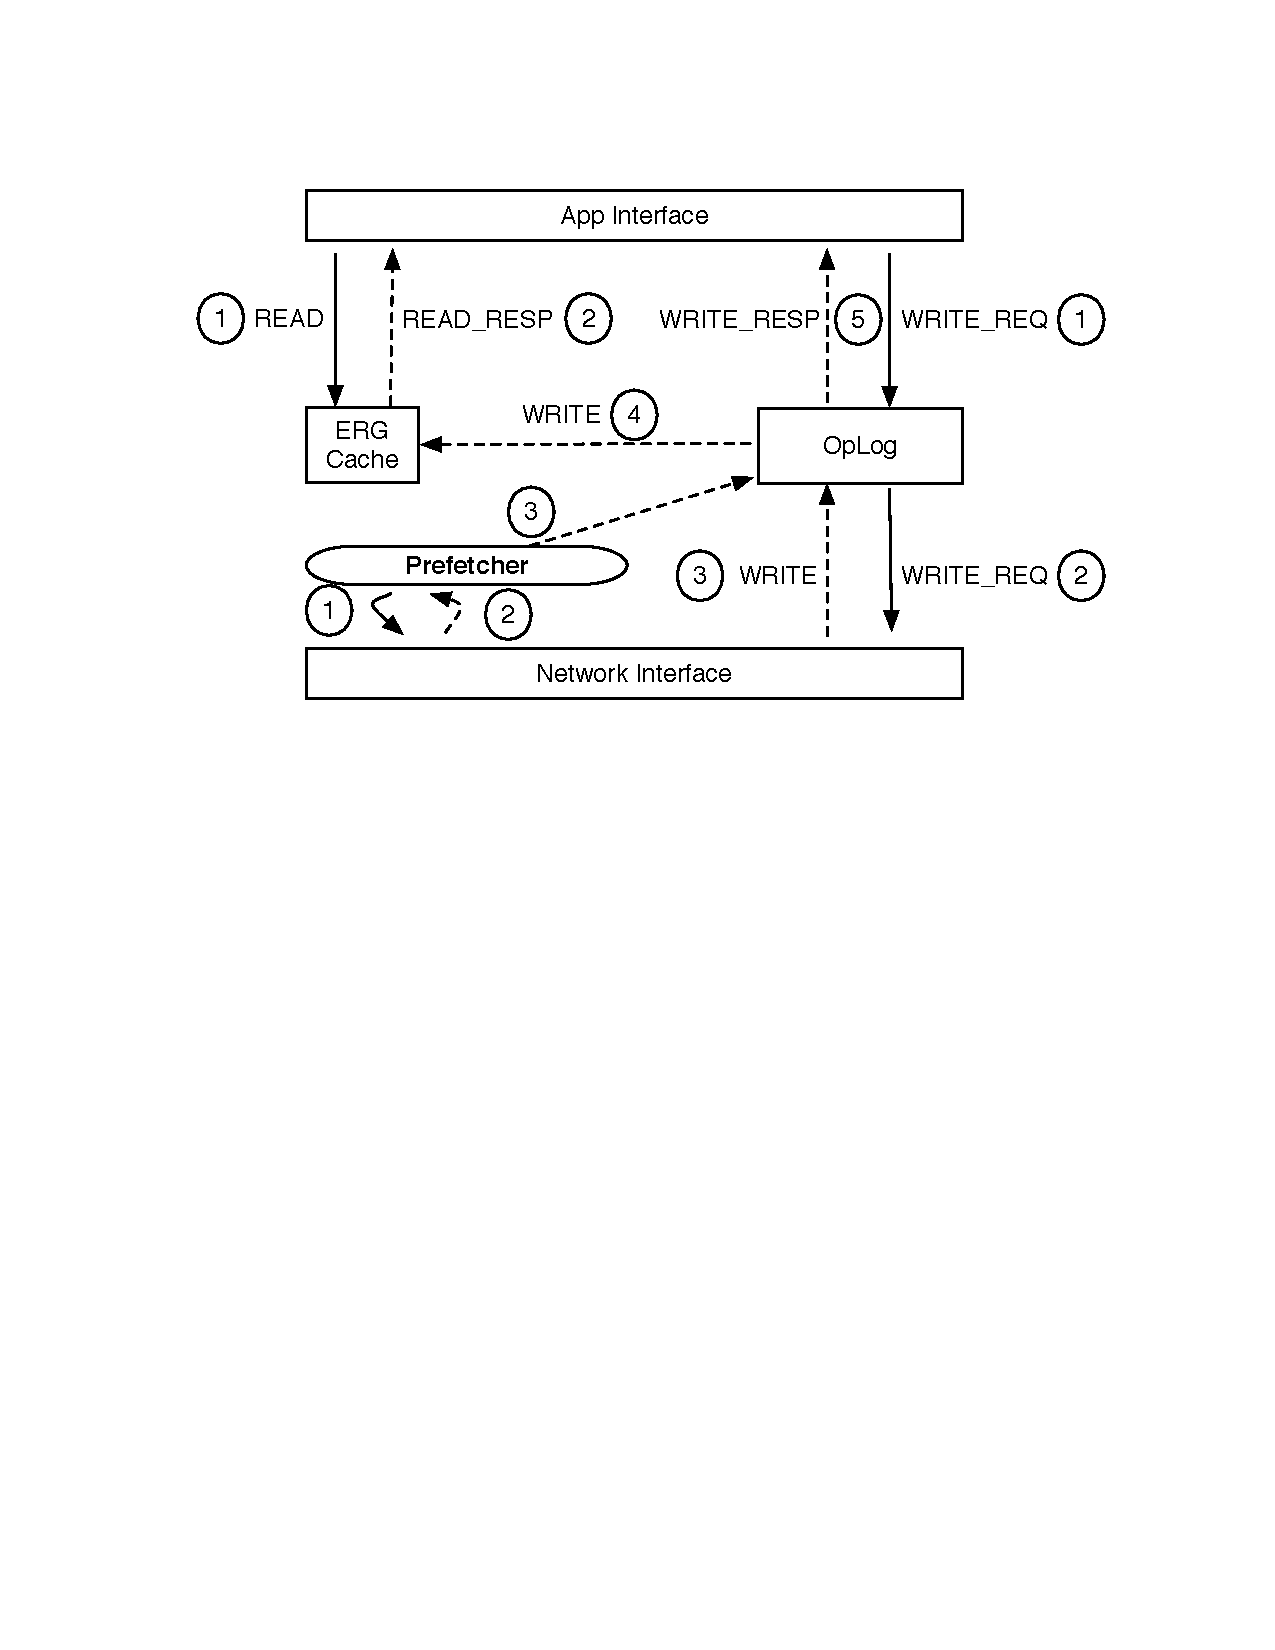
\includegraphics[scale=0.50]{figs/standard_interaction}
\caption{}
\label{fig:interactions}
\end{center}
\end{figure}


\subsection{Swiping gestures}
\label{sec:swipes}

\subsection{Tracking people and things}
There are three major components in our architecture: QR codes, mobile phones, and StreamFS.

How do we evaluate our ability to track people and things?
This is a description evaluation.  We need to describe how the pieces interact.  What will fall out of the description is our strong dependence on occupants/users to give us information about the state of the physical world.  It’ll also fall out that what allows these pieces to fit together is network infrastructure.



\subsection{consistency \& disconnected operations}

The ability to provide real-time analytics for physical data application is driven by 

The consistency and accuracy that we capture about the entities in the world and their relationships and associated metadata.
How those relationships/metadata inform our analytical operations.

Entities in the physical world can be difficult to capture and track over time.  Ideally we’d have a model of the world and the things in it and there would be a mechanism for tracking things that move.  We approximate this mechanism through the combination of QR codes, mobile phones, and people.  Items in the real-world are physically tagged with a QR code that serves as a reference for the “thing” in the physical world.  The mobile phone gives the person a ubiquitous QR code reader.  It also serves to provide the person with services associated with the physical world.

\subsection{Entity-Relationships}
The main aspect we want to capture is entity-relationships between the objects.  Entity relationships are captured through naming and interpreted by the EnergyLens application:

$/path/to/device\_or\_item$

$/path/to/qrc$

$/path/to/space$

$/path/to/taxonomy$

We essentially maintain for separate namespaces and we specify a relationship between them through links between these namespaces.  The relationship is also set by the type of item the path represents.  The types are item, meter, location, system\_device, category, and tag.\\

{\bf Bound-to}\\
When a meter is attached to an item and taking physical measurements associated with that device, we say that the meter is “bound-to” the device.

{\bf Attached-to}\\
When a meter/qr code/item is attached to another meter/qr code/item but NOT taking any physical measurements for that item, we say that the meter/item is “attached-to” the other meter/qr code/item.  QR codes should not be attached to each other and are not accepted by the EnergyLens application.

{\bf Inside-of}\\
When a meter/item is inside a location, we say that the meter/item is “inside-of” that location.

{\bf Type-of}\\
When an item is labeled by as a known, specific, type, we say that the item is a “type-of” thing specified by the its label.


\begin{figure}[htb!]
\begin{center}
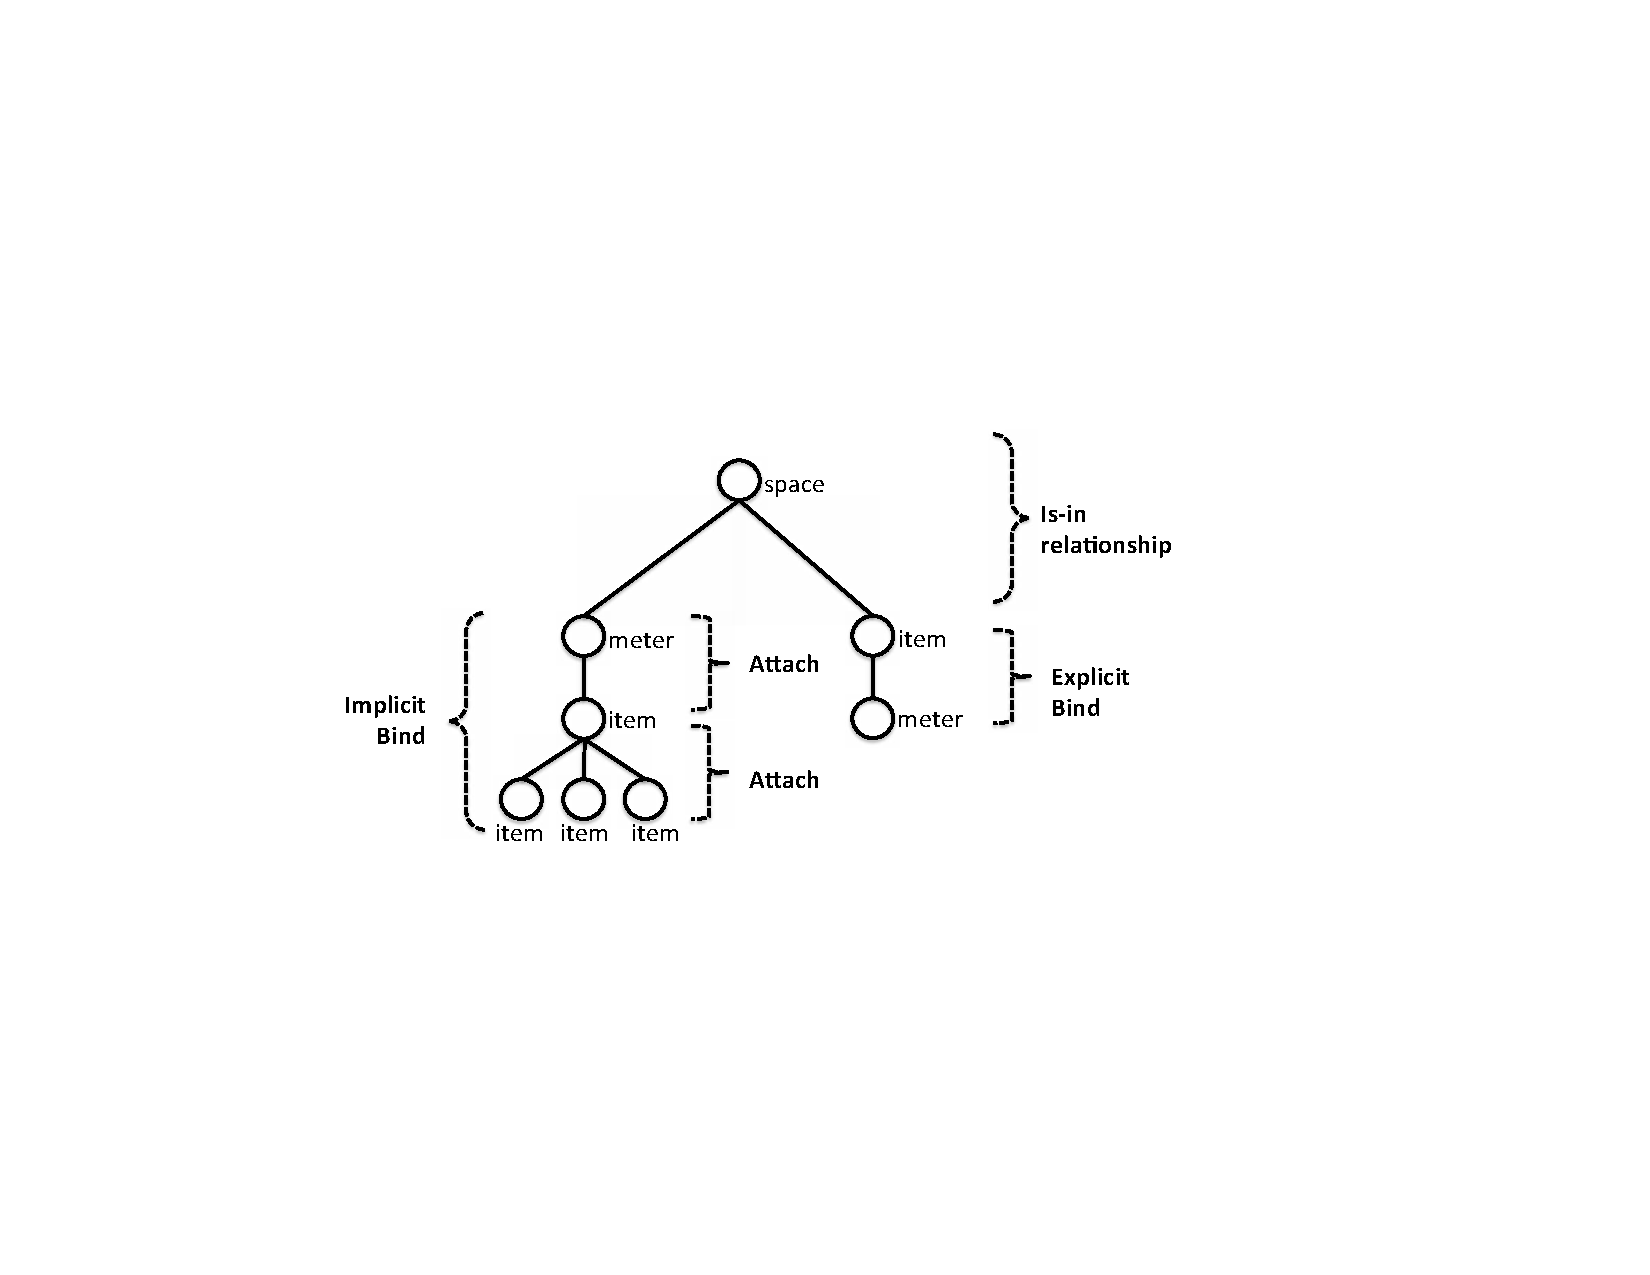
\includegraphics[scale=0.55]{figs/bindattachstructs}
\caption{This diagram shows the relationship capture between the objects and locations in the building for the 
energy audit application.  Children of a space node have an ``is-in'' relationship with the space.  An item
with another item as a child have a ``attached'' relationship and meters attached to items are bound to each other.
Note, this is a \emph{subset} of the relationship diagrams generated across our three applications.}
\label{fig:attachandbind}
\end{center}
\end{figure}

\subsection{Managing consistency while disconnected}

\subsubsection{Caching}
Although network connectivity is theoretically ubiquitous, in practice, this is not always the case.  In order to enable updates while disconnection we need to cache as much of the relevant deployment state as possible.

\subsubsection{Pre-fetching \& The state-change stream}
We should pre-fetch, as the tags inform us about what the user might access next.  What are some things to pre-fetch?  All the paths from the current root to the leaves.  We should also fetch the object associated with each file and for streams, we should fetch 1 hours’ worth of data.  In most cases this means fetching about 200-400 KB of data.

\begin{figure}[htb!]
\begin{center}
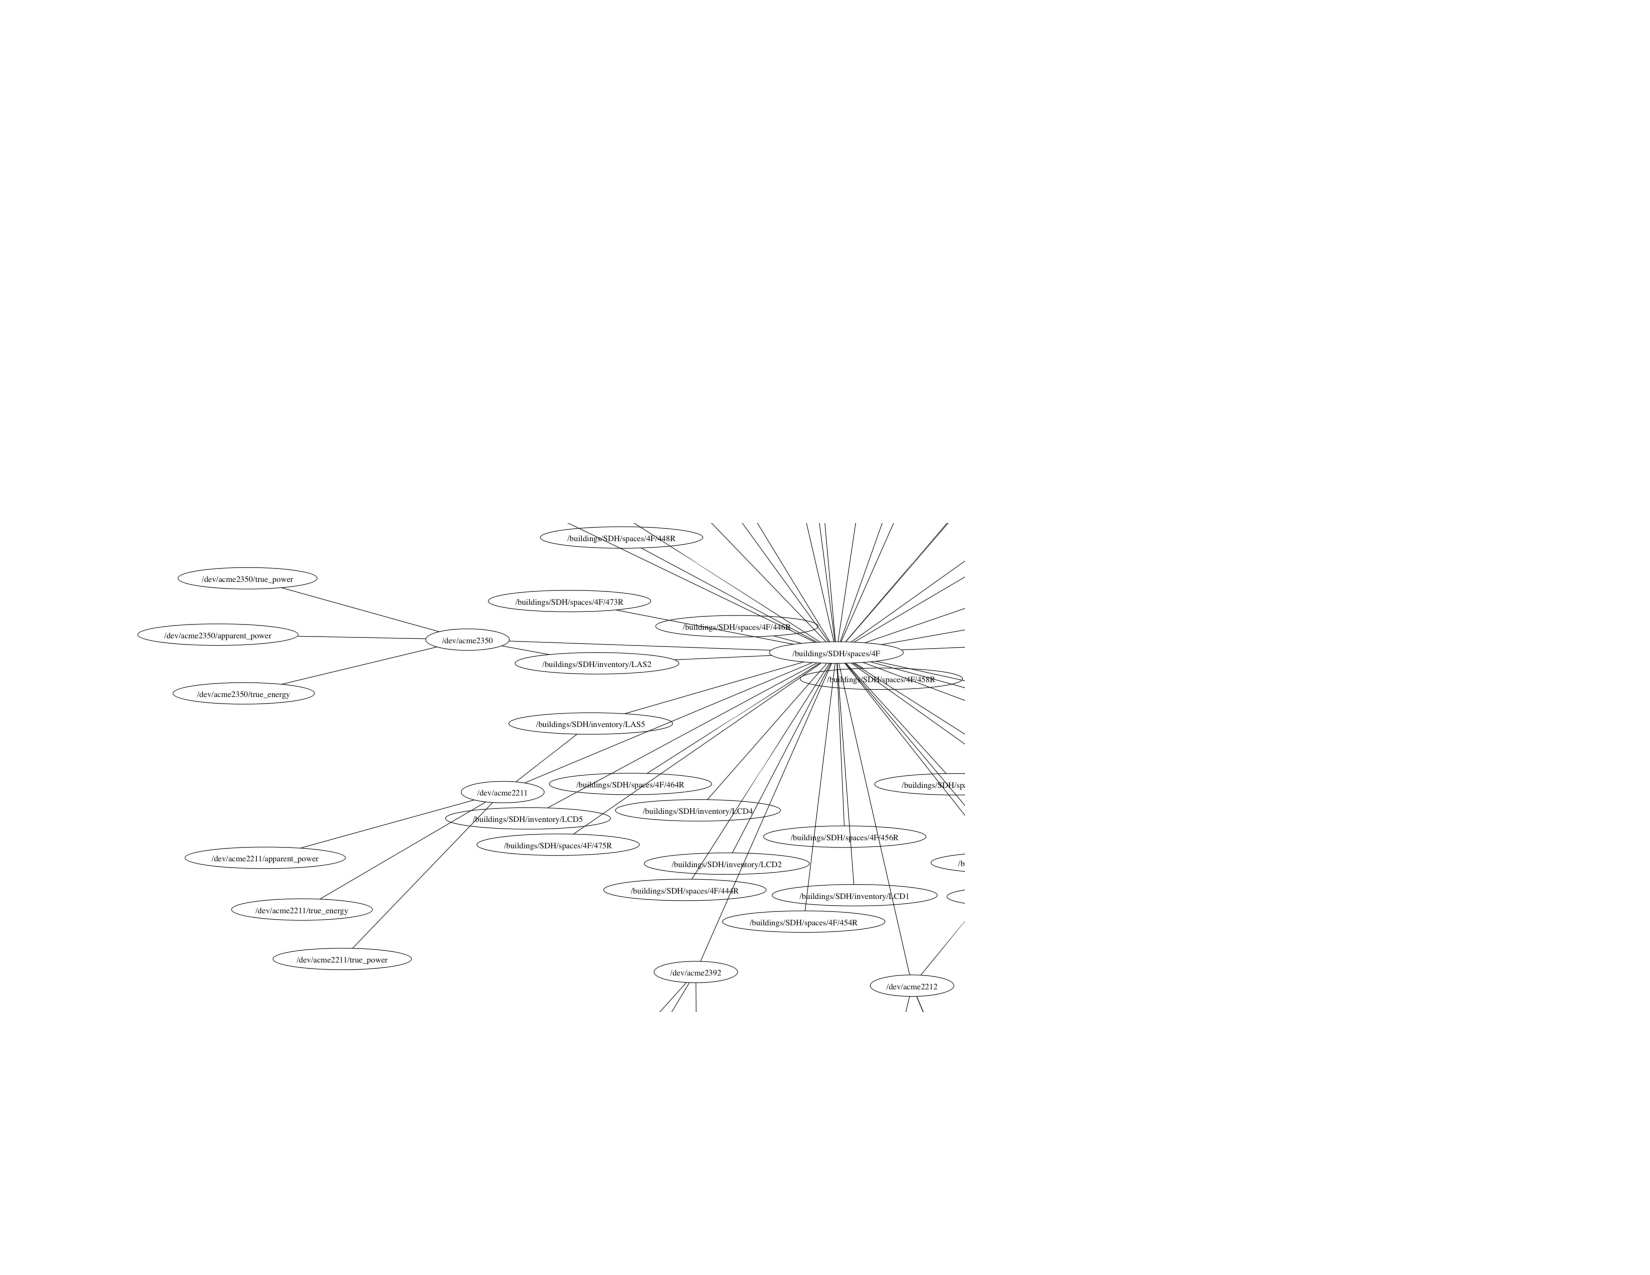
\includegraphics[scale=0.55]{figs/SDH_4F_ERG_closeup}
\caption{A portion of the prefetched entities on the a single floor in our building.  This shows a snapshot of the entity-relationship
graph for that floor.  Each node, link, and associated content is prefetched when the user swipes the floor
tag or anything on that floor.}
\label{fig:sdh_4f_erg}
\end{center}
\end{figure}

\subsection{Conflict resolution}
All transactions are processed in timestamp order, to some rough approximation of the time that the transaction would have been committed.  When a transaction with an earlier timestamp than the last committed transaction is offered, the EnergyLens transaction manager checks if the current transaction conflicts with any previously committed transaction.  This is done by checking if the files that are touched overlap with a transaction that touches the same files and has a transaction timestamp that’s later than the current transaction being offered.  If so the transaction manager rolls back the state of StreamFS, only for the affected files, back to the last transaction before the last commit.  It then commits the offered transaction, adds it to the transaction log, and replays the transaction that was rolled back.  If the operations of the replayed transaction are no longer valid, the transaction fails silently.  Failing silently is acceptable in this context because we want to capture the latest state of the world.  By rejecting the transaction, we are assuming that it was based on false assumptions about the state of the world.  We believe this assumption to be true in most cases.


\subsection{Maintaining, representing, and using physical state and inter-relationships}
In order to provide relevant services, we need to capture the state of the physical environment within the building.  By “relevant”, we mean based on context and inter-relationships.  What are “the relevant services” we’re talking about?

\begin{itemize}
\item Energy analytics on the physical world.
\item How much does this floor consume?
\item What fraction of that is going to the various energy-related categories?  plug-load, hvac, lighting.
\item Personalized energy analytics.
\item Access the the control interface for the physical world.
\end{itemize}

\subsubsection{General approach}
Our approach is to abstractly represents things in the environment as logical entities and to capture their inter-relationships through an entity-relationship graph.  We use the entity relationships to track where objects and things are in the environment, which helps us maintain a more consistent view of the world.  We also use  it to inform our analytical approach and our choice of services to display.

\subsubsection{Consistency management}
Connecting the various components requires ubiquitous connectivity.  Although connectivity is available through the building and the access-point deployment is engineered to minimize dead spots, disconnections still occur (timeout, dead-spots, unsuccessful handoffs).  So, we need to design the system to deal disconnect operation.

Evaluation will be of a protocol description and design rationale described in detail here.
What’s the evaluation exactly?

\begin{enumerate}
\item Time to download the associated contextual information from StreamFS: files, metadata information, data**
\item Conflict resolution examples**
\item Optimizations: Pre-fetching measurements**
\end{enumerate}

\subsection{Real-time analytics}
Discussion.  What to measure here?  Perhaps we discuss the relevant real-time analytics we run?  Will there be space?  For buildsys, include a half page talking about some of the analytics.
% Pub/sub architecture
% time decoupling
% variable time-decoupling achieved through the datastore as a buffer
% synchronization decoupling
% Either the publisher or subscriber run asynchronously.
% space decoupling
% The subscriber doesn’t have an explicit reference to the publisher.
% Programming model for real-time data
% Naming/tagging streams
% Dealing with dynamism through tagging
% Built-in functions for physical data
% heat modeling
% electrical modeling
% mathematical modeling

% Security and privacy
% Discussion.  Various topics related to StreamFS here.  Also some topics related to managing security in StreamFS for doing control.  Include another half page, perhaps.


% * Experiment that we need to run.\\
% ** Code that needs to be written and experiment that needs to be run
\section{Evaluation}
\label{sec:eval}
In this section we measure prefetch download times and discuss strategies for providing scalability.  We also
look at the transaction manager and evaluate conflict resolution times.

% \begin{figure}[htb!]
% \begin{center}
% 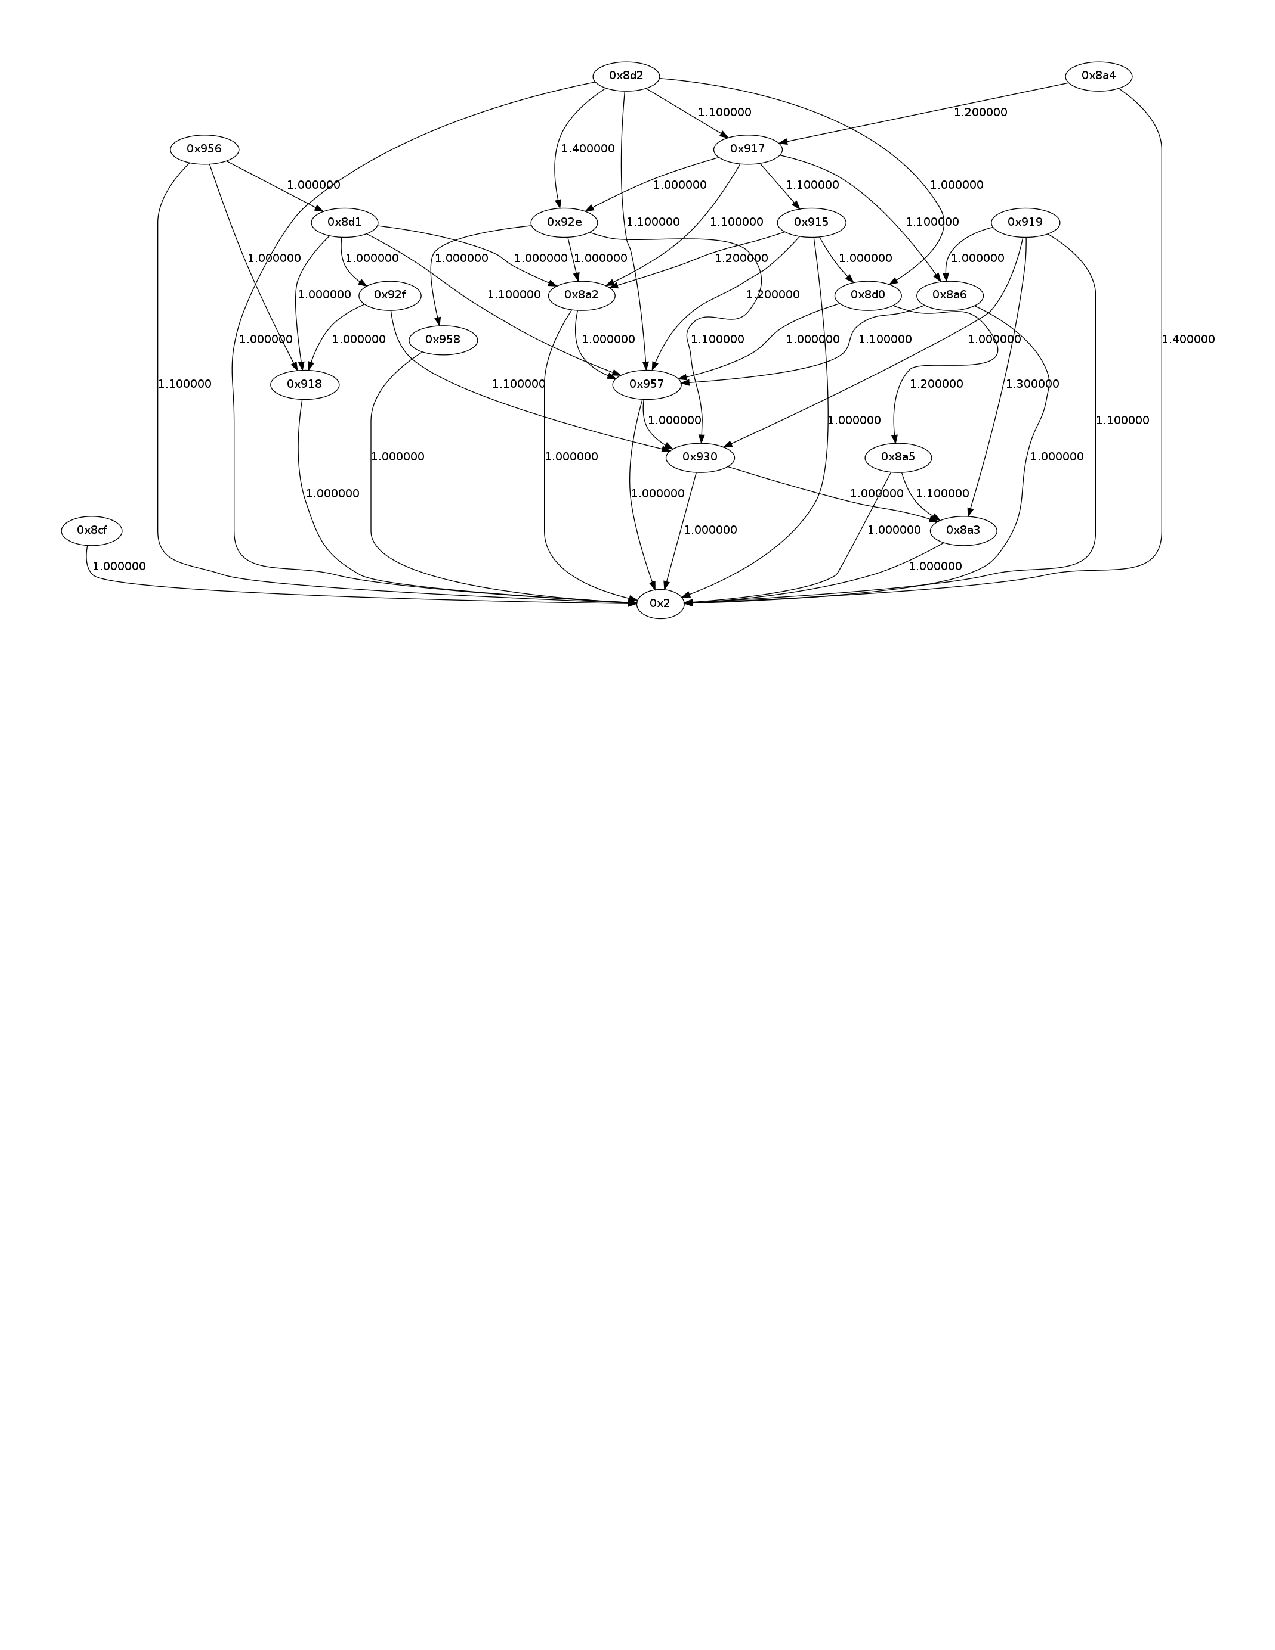
\includegraphics[scale=0.4]{figs/acmenetwork_SDH_4F}
% \caption{}
% \label{fig:acmenetwork_SDH_4F}
% \end{center}
% \end{figure}


\subsection{Prefetching}
Prefetching occurs when a user enters a new floors, as detected by a floor scan or an item
scan.  Table~\ref{tab:prefetchtimes} shows that the prefetch times scale linearly with the number of
items (and data) to prefetch.  Each node holds approximate 100 bytes or information and for
a 20-node deployment of power meters, producing 100 bytes of data per stream (3) every 20 seconds, we fetch 
approximately 1 MB of data.

These prefetch times are non-trivial to deal with, especially since they cause the phone application to slow down
until the data received and loaded into the local cache.  The overhead is dominated by the query in StreamFS that 
constructs the entire sub graph to send to the application.  For future work,  we are will implement a
callback facility and pass the application a reference to it.  The app can then periodically check back until
the query completes and the data is ready to be downloaded.  We can also include partial responses to the query
in the prefetch loop response.  This also allows user to continue using the application without any frustrating waits.

% \subsection{Log dump measurements}
\begin{table}
\begin{center}
  \begin{tabular}{| r | c  c | }
    \hline
    {\bf No. nodes } & {\bf Fetch time (sec) } & {\bf Std. Error (sec)} \\ \hline
    1 & 0.8902 & 0.0756 \\ \hline
    10 & 5.7342 & 1.7087 \\ \hline
    100 & 52.3145 & 14.1146 \\ 
    \hline
  \end{tabular}
\caption{Shows the time to fetch nodes based on the size of the fetch.  The fetch time
increased linearly with the number of nodes.  Caching maintain fetch time near
that of fetching a single node.  A callback is used when cache is invalidated.}
\label{tab:prefetchtimes}
\end{center}
\end{table}


\subsection{Log replay latency}
Table~\ref{tab:optimes} shows the  operation that the transaction manager calls on the StreamFS server.
Log replay and transaction processing is entirely dependent on the time to execute these operations on StreamFS.
There are two types of transactions, a \emph{move}, a \emph{un/bind}, \emph{un/attach}.  A move is a combination
of a `delete' and a `create link', a bind is a `create link' and an `update tags', an unbind and unattach is a
`delete' and `undate tag'.  The transaction latency is the sum of these operations.  By far the most expensive
operation is a `create node' operation.  This occurs when a user adds a new item/space/person to the graph.
The time to apply the operation scale linearly with the size of the logs.  

All logs dumps are processed sequentially.  However, for future work we look to parallelize processing into
parallel processes updating different portions of the graph.  For example, log updates rooted at different floors
could occur simultaneously.




% The global transaction manager implements three main high-level operations -- rollback, apply, and replay.  Our current implementation
% is limited by the time is takes to perform an operation on StreamFS.  Table~\ref{tab:optimes} shows the three 
% main operation that the transaction manager needs to do on the server.
% % Maybe we include another table that talks about the trace we ran through and the conflict times, etc.

% Usually rollbacks consist of \emph{delete} operation and applies consist of \emph{creates}.  In a worst-cases analysis
% of performance we expect the total conflict resolution time to be roughly bounded by
% $rollback\_time + apply\_time + replay\_time$, since $replay\_time=3 X rollback\_time$ and apply\_time is negligible, 
% the total time is approximately $4 X rollback\_time$.  Therefore the overhead is driven by how many new links were created
% that have to be deleted and then re-created.  As an optimization, we limit the scope of a rollback.  The naive
% approach is to blindly undo all operations up to a certain time.  However, we can use the location of the node
% in the ERG to limit the conflict-scope to a sub graph, rather than the entire graph.  The simplest approach is to check if the operation
% on a node either shares an immediate parent with the node that will have an operation undone on it or it the operation
% is on the same node.  By limiting conflict-scope we minimize the number of operation that get execute and, hence, minimize the 
% cost of resolution.



\begin{table}
\begin{center}
  \begin{tabular}{| l | c  c | }
    \hline
    {\bf Operation } & {\bf Avg. exec. time (ms) } &\\ \hline
    fetch & 250 &\\ \hline
    delete & 326  &\\ \hline
    update tags & 267  &\\ \hline
    create link & 250  &\\ \hline
    create node & 1036  &\\ 
    \hline
  \end{tabular}
\caption{Average operation execution time in StreamFS.}
\label{tab:optimes}
\end{center}
\end{table}

% \begin{itemize}
% \item Forwarding
% \item Conflict resolution
% \end{itemize}




% The main driver for the EnergyLens work is to explore the fundamental challenges related to:

% \begin{enumerate}
% \item Tracking people and objects.
% 	\begin{itemize}
% 	\item Through local crowd-sourcing of the tasks to building occupants
% 	\end{itemize}
% \item Maintaining consistency between the relationship between physical items and the entity-relationship graph that represents it.
% \item Providing real-time statistics, information, and processing of energy data related to the building environment.

% 	\begin{itemize}
% 	\item With respect to the occupants
% 	\item with respect to spaces
% 	\item Maintaining security and privacy
% 		\begin{itemize}
% 		\item specifically with respect to personal data and control
% 		\end{itemize}
% 	\end{itemize}

% \end{enumerate}



%\date{14 April 2007}
%\maketitle

% \begin{abstract}
% Despite the growing impact of climate change and energy prices, 
per-capita energy consumption is rising. Part of the problem is visibility. We do not 
have scalable means of observing our energy consumption patterns and determining how to optimize and reduce our
consumption.
Mobile smartphones present a unique opportunity to enable an energy view on the physical world. 
They can bridge the physical world, information infrastructure, and people
through a rich set of sensors, ubiquitous connectivity, and highly personal user interface. 
With QR codes as cheap tags on items and places in the physical world, the
camera becomes a portable scanner in your pocket, in addition to its
traditional functions.  We explore this
unique triple point
and re-examine classical problems of context and consistency management in mobile
systems.  We also examine this combination as it pertains to energy management of physical
devices.  In doing so, we are re-introduced to problems of apportionment and aggregation of sensor data,
except with a continuously changing set of constituents.  We describe our solution in a technique
called \emph{dynamic aggregation} that maintains moving aggregates as the
set of data sources changes over time.  We deployed our system in a 
141,000 square-foot building, tagging 351 items over 139 room across 7 floors.

% When combined with QR codes, the on-board camera provides us with a portable scanner

% The camera,
% when combined with QR codes, gives us a portable scanner and convenient mechanism for tying these world together. 
% In this paper, we describe our system and deployment experience for a mobile phone application the provides 
% user-centric energy-view of the physical world. We describe the challenges, specifically dealing with mobility, 
% and how we address them in a set of three separate applications: an energy auditing application, a 
% device energy scanner, and a personal energy counter. We also introduce a technique called \emph{dynamic aggregation}
% which allows us to seamlessly track the constituents of aggregated energy calculations, as they move from one 
% location to another.

% Despite the recent impact of global warming and a steady increase in energy prices, 
% per-capita energy consumption is rising. Part of the problem is about visibility. We simply do not 
% have any good ways of seeing how we consume energy, and therefore, how to optimize and reduce it. 
% \end{abstract}

% A category with the (minimum) three required fields
%\category{B.0}{Hardware}{General}
%\category{B.4}{Hardware}{Input/Output \& Data Communication}

%\terms{Design, Implementation, Performance, Experimentation}

%\keywords{Churn, Link, Routing, Wireless, Sensor Network, Mote}

%\newpage
% \subsection{Introduction}
The United States leads the world in per-capita energy consumption.
Our electricity use has consistently increased over the last 40 years~\cite{oecd2011} and other parts of the world are rising all 
too rapidly.  With the specter of climate change and the increasing cost of energy, we must explore new
ways for individuals to gain visibility and insight into their energy consumption in order to optimize and reduce it. 
With the increasing penetration of embedded sensors in the environment and
the continued rise in smartphone adoption, we see an opportunity for smartphones to bridge the physical world
to our computational infrastructure and provide an `energy lens' on the physical world.  

We use mobile phones to construct an entity-relationship 
graph of the physical world and combine it with streaming sensor data in order to perform detailed energy-attribution.
We limit the scope of the world to a single building domain.  We have designed and implemented a real-time, mobile energy auditing
application, called the `Energy Lens', that allows us to collect information about 
things throughout the building and how they are related to each other.  For example, computer X is inside 
room Y and connected to meter Z.  Then, we use these relationships to guide our data look-up and analytical
calculations.  For example, the load curve of room Y consists of the sum of all the power traces for loads
inside room Y.  We use the mobile smartphone as the main input tool.  Our work examines \emph{three main challenges} in setting up and 
deploying a real, whole-building infrastructure to support real-time, 
fined grained energy analytics.  

The first challenge is related to tracking and mobility.
The use of mobile phones presents classical, fundamental challenges related to mobility.  Typically, mobility
refers to the phone, as the person carrying it moves from place to place.  However, in the energy-attribution
context, we are also referring to the movement of energy-consuming objects.  Tracking their relationships to spaces 
and people is as important as tracking people.  We describe how we deal with \emph{both moving people and 
moving objects} and show that these historically difficult problems can be addressed relatively easily, if the proper infrastructure is 
in place.  %We provide evidence that the approach is simple, incrementally deployable, and scalable.

The second challenge is about capturing the inter-relationship semantics and having these inform our  analytics.
We adopt the general notion of physical tags that identify objects in the world.  Our system uses \emph{QR codes} to tag things and locations 
in the physical world.  However, \emph{any tag that provides a unqiue identifier for an object could serve the same purpose}.
Once tagged, there are three types of interactions -- 
registration, linking, and scanning -- which establish important relationships.  Registration is the act of creating a virtual object 
to represent a physical one.  Linking captures the relationship between pairs of objects.  Scanning is the act of performing an item-lookup.
Each of these interactions requires a set of swiping gestures.  Linking requires two tag swipes while the other two actions
require a single tag swipe.  Internally, we maintain a \emph{entity-relationship graph (ERG)} of things, people, and locations, that gets
updated through these sets of gestures.

The third challenge is about indoor network connectivity and access.
In order to connect these components, we rely on having `ubiquitous' network connectivity.  However, in practice, network
\emph{availability} is intermittent and our system must deal with the challenges of intermittency.  We discuss how caching
and logging are used to address these challenges.  Moreover, when connectivity is re-established, we must deal with
applying updates to the ERG, as captured by the phone while disconnected.  
% Conflicts can also occur during an update.  For example, the two updates may disagree about which items are attached
% to which meters.  We implement a very simple conflict resolution scheme, described in section~\ref{sec:conflicts}.
% Finally, certain physical-state transitions are represented as a set of updates to the ERG that must be applied 
% atomically.  We implement transactions in the log-replay and transaction manager.
% Our `Energy Lens' system is deployed in a building on our campus.  We discuss
% its architecture and our design choices.  
  
% We also discuss novel strategies for tracking moving people/things and describe how we implement these in our system.  In summary, our work
% makes the following contributions:

% \begin{itemize}
% \item We design and implement a system that captures and combines physical entities, their inter-relationships, and real-time sensor data 
% 		in buildings.% using mobile phones, qr code, and a cloud-based infrastructure.
% \item We observe that certain combinations of swipes give us useful information to set the location of people and things over time.
% 		We codify this observation in our \emph{context-tracker} and use it to maintain consistency between the entity-relationship graph and the 
% 		state of the physical world.  To the best of our knowledge, this is radically different from the approaches in standard 
% 		localization techniques.  However, we argue that it can be used to \emph{enhance} their accuracy and overall performance.
% \item We implement a prefetching algorithm to obtain context-dependent information to both improve performance and
% 		enable disconnected operation.  We also design and implement a log-replay and transaction manager over our data management layer.  We describe how different conflict-resolution policies can be implemented and our rationale for the policies we chose.
% \end{itemize}

% \vspace{0.08in}

% In the next sections we go through a motivating scenario.  We then discuss some related work, followed 
% by the system architecture, evaluation, and future directions.


%
% The marriage of pub/sub, streaming dbms, and filesystems
%


\vspace{+0.5mm}
\vspace{+2mm}
\bibliographystyle{abbrv}
%\scriptsize
\bibliography{references}

\end{document}


